\documentclass{article}
\usepackage[utf8]{inputenc}
\usepackage{graphicx}
\usepackage{float}

\title{Requirement Analysis and Specification Document: bike4share}
\author{Maffioli Sara, Papale Lorenzo, \\ Stucchi Lorenzo \& Vaghi Federica}


\begin{document}

\maketitle
\tableofcontents

\newpage

\section{Introduction}
\subsection{Purpose}
The aim of the project is to develop a web application called “bike4share” for a bike sharing service in order to guarantee to the user a web service to search for the availability of bikes and free stalls around his position or the desired location in the city. The web application must ensure the technician to have a private section showing analytic graphs and statistics on the bike flow in real time.
\subsection{Scope}
The “bike4share” application must provide a service of registration and of log-in both for user and technician. The user information related to availability and location of bikes and free stall are shown by a web map, one of main functionalities of “bike4share”. The user can have access to premium functions through the registration on web service, for example the mean of the available bikes and stalls in a certain hour that can be selected or the notification of availability or full over a certain level. There is also a mail service to ensure the recovery of the forgot password.
“bike4share” must provide to the technician a dedicated analytics section, in order to analyse and study the bike stations trends in real time and also during a set span of time. This analytics section guarantees statistic, like mean of bikes used during a certain period, and graphs showing trends, relying on the data stored in a designed database.
\subsection{Definitions, acronyms, abbreviations}
---
\subsection{Reference documents}
---
\subsection{Overview}
The RASD document is structured in four main chapters, i.e. Introduction, Overall Description, Specific Requirements and Appendices. The next chapter, “2 Overall Description “, is divided in five subchapters devoted to the description of the external interfaces and shared phenomena, summary of the major product functions, user characteristics, constraints and last one devoted to assumptions and dependencies.
In the third chapter, ”3 Specific Requirements ”, is presented a full list of the requirements and the associated use cases. Always in this section two subchapters are present: one devoted to the specifications about the design constraints, such as standards compliance and hardware limitations and the other one is focus on the software system attributes, i.e. reliability, availability, security, maintainability and portability.

\section{Overall Description}
\subsection{Product perspective}
Our web application “bike4share” will work thanks to several components supporting it. As shown in the scheme in Figure \ref{fig:schema}, we can recognise three levels of the system: Data, Software and User. 
Starting from the bottom and considering the inputs, Data are retrieved from two Databases, one for the registered users and technicians and one for the information regarding the bike stations. 
The outputs of “bike4share”, instead, are the visualisation of a map showing the bike stations with the relative information (bikes and free stalls) and the visualisation of statistics (only for technicians and premium users). 
The third level is the one regarding the user, capable of viewing the map to obtain the information, and the technician, who can perform API request to analyse data and statistics. Both the actors can perform their purposes accessing the page through the browser. 

\begin{figure}[h]
    \centering
    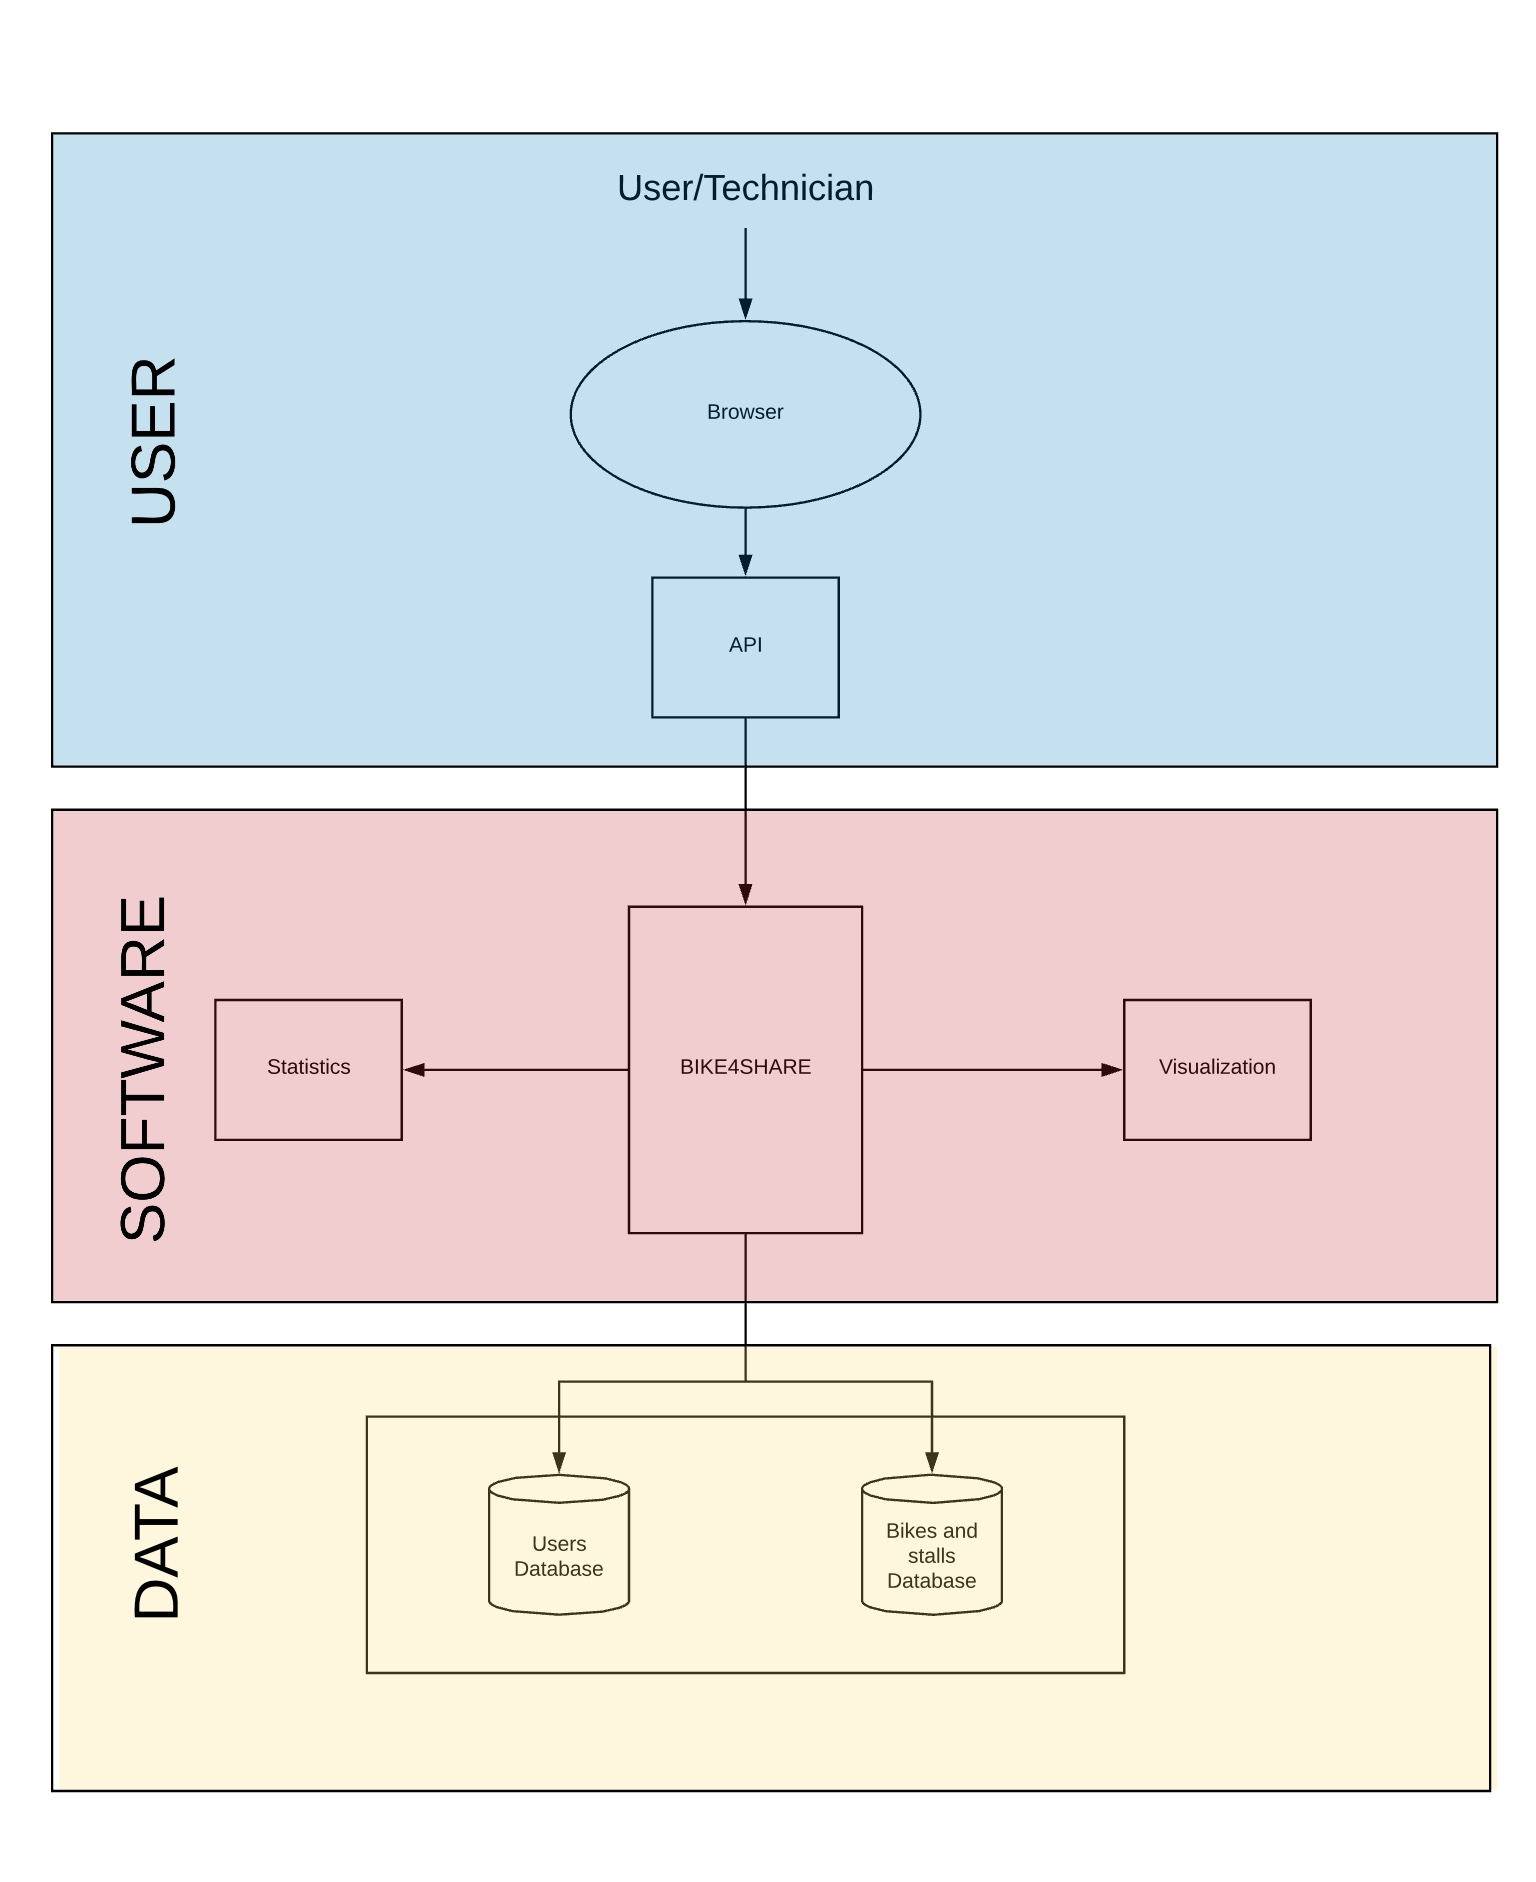
\includegraphics[width=0.75\linewidth]{image/overallview.PNG}
    \caption{Overall view of "bike4share" system}
    \label{fig:schema}
\end{figure}

\subsection{Product functions}
"bike4share” provides different functions to different type of users. 
The basic function provided to all the users is a web page with a map with the position of all the bike stalls and the realtime number of bikes present in each stall and the number of free ones.
If the user logs into the system, after the registration, can access to extra functionalities that can help the usability of the app by the user. Premium functions are the displaying of the position of the user on the map, to help the user to see the nearest station, and also a list of the stations will appear near the maps, if the users doesn’t allow to access to the position or this feature is not available for the user system, the user can insert the address or select the position on the map. Another function that a user can use is for estimating the mean number of bikes available and free stalls in a certain hours selected by the users. 
There is also a specific section of the application “bike4share” devoted to the technician’s use. The technician is requested to complete the registration and log-in to have access to the specific section, in which analysis instruments and graphical statistic tools are provided. 
\begin{itemize}
    \item Trend of the bikes usage during a selected span of time;
    \item Average of the bikes during the day/week/month;
    \item The most used bike stalls (histogram) during the day/week/month
\end{itemize}

\subsection{User characteristics}
\begin{itemize}
    \item \textbf{Registered user}: a user that is registered yet and that wants to access the “bike4share” WebApp services in order to use the premium functions available on the application, it could be a person that uses this service frequently. 
    \item \textbf{Not registered user}: a user that isn’t registered yet and that wants to access the “bike4share” WebApp  services in order to use the basic functions available on the application, it could be a person that  doesn’t use this service frequently or a new user that wants to start an approach to this service and try it for the first time.
    \item \textbf{Technician}: a person who is authenticated thanks to specific credential given by the master of the service and  who has been granted supervising permissions. He/she is allowed to view, analyze, access statistics and aggregated information about the “bike4share” WebApp services.
\end{itemize}

\subsection{Constraints}
\subsubsection{Regulatory Policies}
“bike4share” relies on map applications as Google Maps, Bing  and so it must respect their market policies.

\subsubsection{Interfaces to other applications}
“bike4share” interacts with a database system.

\subsubsection{Parallelism}
“bike4share” must support parallel operations coming from both user and technician on the same database.

\subsection{Assumptions and Dependencies}
\begin{itemize}
    \item Non registered user must have a smartphone or a computer with internet connection available to exploit the “bike4share” services;
    \item Registered user needs a smartphone or a computer with internet connection and active GPS in order to use the premium functions available on the application, e.g. localization function;
    \item Non registered technician must have a smartphone or a computer with internet connection available to register on the application and then access the devoted section;
    \item Registered technician is required to have a smartphone or a computer with internet connection in order to access the devoted section of the application;
\end{itemize}

\section{Specific Requirements} 
\subsection{External Interface Requirements}
\subsubsection{User Interfaces}
---
\subsubsection{Hardware Interfaces}
---
\subsubsection{Software Interfaces}
---
\subsubsection{Communication Interfaces}
---

\subsection{Functional Requirements}
It is possible to define different type of users, in particular in this document the Log-In case, the Registration case, the Forgot Password case,the Data Visualization (NO PREMIUM) case, the Data Visualization(PREMIUM) case, the Registration of the Technician case, and the Technician Analysis case are shown in their details.

\subsubsection{\textbf{USE CASE}: Log-In}
\begin{enumerate}
\item Participating actors: 
\begin{itemize}
    \item registered user
    \item WebApp
\end{itemize}
\item Entry Condition: 
\begin{itemize}
    \item user wants to access to premium functions (so have to log in)
\end{itemize}
\item Flow of events: 
\begin{itemize}
    \item user enters in the page and puts the username
    \item user inserts also the password
\end{itemize}
\item Exit Condition: 
\begin{itemize}
    \item user is logged in the WebApp
\end{itemize}
\item Exceptions
\begin{itemize}
    \item the username doesn’t exist so the system shows an error and proposes the user to register
    \item the password is wrong so the system shows an error and proposes to reinsert the password and shows the propose to change the password 
\end{itemize}
\end{enumerate}

Scenario 1: “bike4share” Log-In \\
Mario needs a bike to go back from his position to his home near to Parco Sempione. He decides to open the “bike4share” WebApp in order to know if there are some bike stalls available near to his position. 
Pippo is registered yet so he has to insert his username and his password, in this way he can access to the PREMIUM FUNCTION. 
He is asked to allow the application to use his position and after that he can check the bike stalls distribution on the map. 
If Mario doesn’t want to allow the usage of his position or if this feature is not available for his system he can insert directly the address and the list of the station will appear on the screen. Now Mario can go by foot to the nearest stalls and finally come back home riding a bike.

\subsubsection{\textbf{USE CASE}: Registration}
\begin{enumerate}
\item Participating actors: 
\begin{itemize}
    \item new user
    \item WebApp
\end{itemize}
\item Entry Condition: 
\begin{itemize}
    \item new users want to register in order to be able to use the premium WebApp functionalities
\end{itemize}
\item Flow of events: 
\begin{itemize}
    \item new users have to sign in
    \item new users have to insert their e-mail
    \item new users can set an username
    \item new users can set a password
\end{itemize}
\item Exit Condition: 
\begin{itemize}
    \item new users are registered
\end{itemize}
\item Exceptions
\begin{itemize}
    \item the username exists yet so an error is shown and it is proposed to change the previous username
    \item the format of the mail is wrong so the system requires to correct it and insert a valid one.
\end{itemize}
\end{enumerate}

Scenario 2: “bike4share” Registration \\
Luca wants to take the train starting from the Cadorna railway station at 13.00 p.m. but he knows that he is late and he can’t arrive in time if he goes by foot. Fortunately he works in L.go Greppi near a bike stall so one of his colleagues suggest him to use the “bike4share” WebApp in order to reach the station by bike. Luca tries to use the “bike4share” WebApp in order to discover the list of the stalls near the Cadorna railway station where he could left the bike taken from the L.go Greppi bike stall. 
He hasn’t so much time and the manual research of his position offered by the BASIC FUNCTIONS of “bike4share” aren’t enough so he needs to access to PREMIUM FUNCTIONS.
He tries to access directly to the “bike4share” WebApp PREMIUM FUNCTION but the user name doesn’t exist so the system shows an error and propose to register.
As new user Luca has to sign in by compiling the form with his correct format e-mail, an user name and a password. 
If the user name that Luca has inserted is chosen yet an error is shown and it is proposed to change the previous set name, otherwise the registration is successfully completed.
Now Luca can access to the the “bike4share” WebApp PREMIUM FUNCTION and check the stalls’ list near the Cadorna railway station.

\subsubsection{\textbf{USE CASE}: Forgot Password}
\begin{enumerate}
\item Participating actors: 
\begin{itemize}
    \item user
    \item WebApp
\end{itemize}
\item Entry Condition: 
\begin{itemize}
    \item user forgot the password and wants to restore it
\end{itemize}
\item Flow of events: 
\begin{itemize}
    \item users have to put the username 
    \item users have to put the e-mail associated to the account 
    \item the system sends back the old password using the user e-mail
\end{itemize}
\item Exit Condition: 
\begin{itemize}
    \item user has into his mail the password
\end{itemize}
\item Exceptions
\begin{itemize}
    \item the users don’t remember anything about the previous registration so it is necessary to do again the registration processes
\end{itemize}
\end{enumerate}

Scenario 3: “bike4share” Forgotten Password \\
Lucy bought a ticket to go to the cinema tonight for a new Marvel’s film. She decides to go with the train but the show finishes at midnight so there won’t be the trains for the return. 
she wanted to save money because she has already spent a lot for the show ticket so instead of booking a taxi she tries to open the “bike4share” WebApp from the internet cafè near the cinema. lucy can’t remember the password of her account but she still need to come back home and so she wants to restore her password. 
The system requires to insert the user name, the e-mail address associated to the account and at this point the system can send back the old password to the given e-mail address.
 At this point Lucy can walk to the chosen bike stall  and she finds another girls that is trying to remember her credential but unfortunately this girl can’t remember anything of the previous registration so she has to do again the registration process. Lucy helps her to find another stall near her house and at the end they both can pick up a bike and came back home.


\subsubsection{\textbf{USE CASE}: Data Visualization (BASIC FUNCTION)}
\begin{enumerate}
\item Participating actors: 
\begin{itemize}
    \item user not registered
    \item WebApp
    \item “background” map application as Google Maps, Bing
\end{itemize}
\item Entry Condition: 
\begin{itemize}
    \item user wants to see on a map how many bikes and how many stalls are available for each station.
\end{itemize}
\item Flow of events: 
\begin{itemize}
    \item user manually checks in the map where are the stations and the number of free bikes/stalls that are available in that place in real-time
\end{itemize}
\item Exit Condition: 
\begin{itemize}
    \item If there is availability of bikes in the interested area at this time (estimation of return time of the bike if it exists?) and the user successfully goes to the bike station, otherwise the user closes, logs out  the application.
\end{itemize}
\item Exceptions
\begin{itemize}
    \item if the localization doesn’t work the logged user can insert the address and find the position
    \item maps providers crash
    \item server doesn’t work
\end{itemize}
\end{enumerate}

 Scenario 4: “bike4share” Data Visualization (BASIC FUNCTION) \\
Max is a student and he has to go to the university but in the morning there’s an underground line services strike so he wants to see on the map how many bikes and how many stalls are available in real-time near Centrale underground station where he is forced to stopped and near his university in Piazza Leonardo which he has to reach. 
Thanks to “bike4share” WebApp BASICS FUNCTION he can manually check on the map that there are 2 bike stalls near the underground station and many different bikes available but there aren’t any stalls near Piazza Leonardo so he close the application and maybe he has to find another way to reach the university.


\subsubsection{\textbf{USE CASE}: Data Visualization (PREMIUM)}
\begin{enumerate}
\item Participating actors: 
\begin{itemize}
    \item user registered
    \item WebApp
    \item “background” map application as Google Maps, Bing
        \item Bike Data (API database)
\end{itemize}
\item Entry Condition: 
\begin{itemize}
    \item user, considering his position, wants to see on a map how many bikes and how many stalls are available for the nearest station and for all the other ones
\end{itemize}
\item Flow of events: 
\begin{itemize}
    \item user, depending on his position, checks in the map where are the stations and the number of free bikes that are available in this place in real-time
    \item user logged in the system and access to premium functions involves tools like:
\begin{itemize}
        \item the mean of the available bikes and stalls in a certain time 
        \item notification of availability or full over a certain level
        \item from position appears a list of the bike stalls available and occupied
\end{itemize}
\end{itemize}
\item Exit Condition: 
\begin{itemize}
    \item If there is availability of bikes in the interested area at this time (estimation of return time of the bike if it exists?) and the user successfully goes to the bike station, otherwise the user closes, logs out the application
\end{itemize}
\item Exceptions
\begin{itemize}
    \item localization doesn’t work so logged user can insert the address and find the position or add a point in his position
    \item user forgets the password (credentials) -> send a mail
    \item maps providers crash
    \item server doesn’t work
\end{itemize}
\end{enumerate}

Scenario 5: “bike4share” Data Visualization (PREMIUM FUNCTION) \\
Mary wants to invite some of her friends to Parco Sempione in order to spend a funny day together by riding the bikes and to escape from the hottest day of the season, 
She decides to check on “bike4share” WebApp, considering their positions, how many stalls and how many bikes are available in real time for the nearest station of her house and for all the other stations near her friends and Parco Sempione; she can check both looking directly on the map or, if the GPS system doesn’t work, she can insert the address and find the position.
Mary as registered user is logged in the system and she can access to PREMIUM FUNCTIONS that allow her to use some interesting tool such as the mean of available bikes and stalls in a certain time, the notification of full over a certain level of the stalls and a list of available/occupied stalls  in order to plan a perfect day for her friends.

\subsubsection{\textbf{USE CASE}: Registration of the Technician}
\begin{enumerate}
\item Participating actors: 
\begin{itemize}
    \item new user
    \item WebApp
\end{itemize}
\item Entry Condition: 
\begin{itemize}
    \item Technician register for the first time
\end{itemize}
\item Flow of events: 
\begin{itemize}
    \item technician receives a fixed username by mail
    \item technician inserts the username
    \item technician has to insert his e-mail
    \item technician can set a password
\end{itemize}
\item Exit Condition: 
\begin{itemize}
    \item technician is registered 
\end{itemize}
\item Exceptions
\begin{itemize}
    \item the format of the mail is wrong so the system requires to correct it and insert a valid one
\end{itemize}
\end{enumerate}

Scenario 6:  “bike4share” Registration of the Technician \\
Orazio is a new technician that is been assigned to the “bike4share” WebApp data management and data analysis and he must register himself for the first time. 
Orazio has received a fixed username by e-mail from the system and he logs in for the first time with the given username, after that he has to compile the appearing form with his e-mail address and he has to set a password.
At the end of the procedure if the e-mail address is formally correct the new technician is successfully registered otherwise an error is shown and the system requires to insert another valid e-mail address. 


\subsubsection{\textbf{USE CASE}: Technician Analysis}
\begin{enumerate}
\item Participating actors: 
\begin{itemize}
    \item technician
    \item “background” map application as Google Maps, Bing
    \item Bike Data (API database)
\end{itemize}
\item Entry Condition: 
\begin{itemize}
    \item technician wants to analyse the distribution of the bike stations and study their trend
\end{itemize}
\item Flow of events: 
\begin{itemize}
    \item technician logs in the system to access to a private section
    \item then technician can check the trend of a bike station in real time and the trend during a time span that can be set
\end{itemize}
\item Exit Condition: 
\begin{itemize}
    \item technician wants to stop the analysis and logout
\end{itemize}
\item Exceptions
\begin{itemize}
    \item user forgets the password (credentials), so the service for forgot password can be activated
    \item maps providers crash
    \item server doesn’t work
\end{itemize}
\end{enumerate}

Scenario 7: “bike4share” Technician Analysis \\
Clara is an expert technician that wants to analyze the distribution of the bike station and study their trend in order to obtain more information related to the usage of the services offered by the “bike4share” system WebApp for her client.
She has to logs in the system and make the access to a private section, reserved only for the technicians, where Clara can check the trend of a specific bike station in real time or set a time span in which she is interested in. For example she can check if during the lunch time there are enough bikes available in the stall of P.za S.Ambrogio, near the university, in this way she can consider if it’s better to increase the number of bikes in that station or not in order to be able to offer a better service.
At the end of her analysis Clara can close the application and shows to her bosses the results that she has obtained.
If some technician forgets the credentials it is possible to activate the “Forgotten Password” service as it is described in the Scenario 3: “bike4share” Forgotten Password.

\subsection{Performance Requirements}
---
\subsection{Design Constraints}
PostgresSQL is used in order to manage the databases
Python is used in order to perform the outputs using the available libraries. 
Libraries as Shapely, Padas and Geopandas are used in order to build the map and to manage a background map with the entities that we want to represent.
Libraries as Numpy, Seaborn and Bokeh are used for the visualisation of the statistics. 
---
\subsubsection{Standards compliance} 
---
\subsubsection{Hardware limitations etc.}
---
\subsection{Software System Attributes}
\subsubsection{Reliability}
---
\subsubsection{Availability} 
---
\subsubsection{Security}
---
\subsubsection{Maintainability}
---
\subsubsection{Portability}
---
\subsection{Other Requirements}
---
% \section{Appendices}

\end{document}
